\section{Evaluation}

%%%%%%%%%%%%%%%%%%%%%%%%%%%% Evaluation Setup %%%%%%%%%%%%%%%%%%%%%%%%%%%%
\begin{figure*}[t]
\centerline{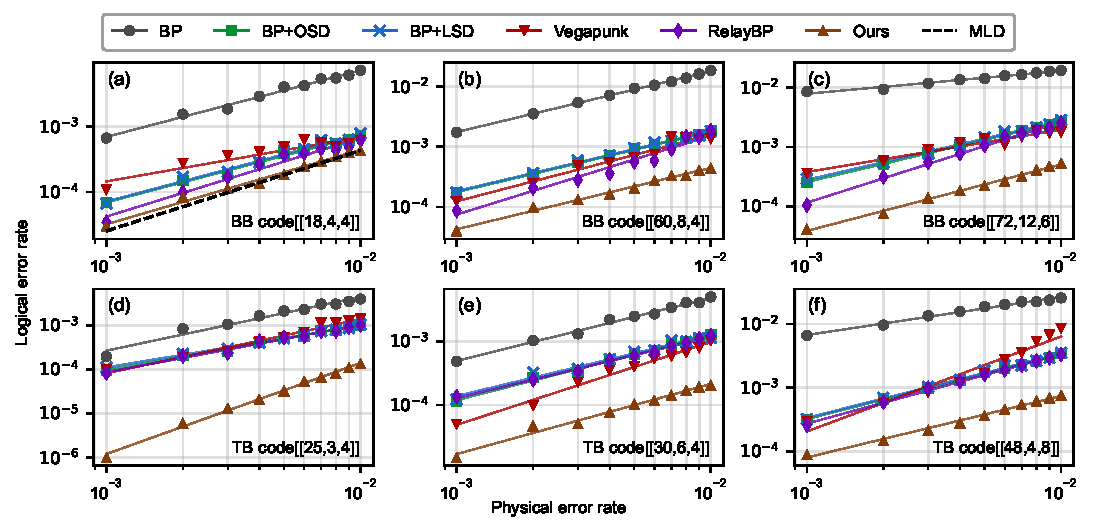
\includegraphics[width=\textwidth]{figures/Evaluation/LER_exp_mld.pdf}}
\vspace{-0.4cm}
\caption{The logical error rates (LER) for BP \cite{bp}, BP+OSD-CS(7) \cite{bposd}, BP+LSD \cite{bplsd}, Vegapunk \cite{zhou2025vegapunk}, RelayBP \cite{relaybp}, \papername, and Exact MLD, respectively. The physical error rate $p$ ranges from $1 \times 10^{-3}$ to $1 \times 10^{-2}$. We evaluate the LER using a depolarizing noise model.}
\vspace{-0.2cm}
\label{fig:LER_exp}
\end{figure*}

\subsection{Evaluation Setup}

\textbf{Metrics.}
We quantify the effectiveness of \papername through three critical performance metrics: (1) the logical error rate (LER), (2) the decoding latency, and (3) tensor compression.
Upon accumulating $d$ rounds of syndromes (where $d$ is the code distance), \papername applies a correction operation to the logical qubit and subsequently measures its state. A logical error happens if this final logical measurement diverges from the pre-initialized state. The decoding process is iteratively executed numerous times under a defined noise model, with each syndrome generated using the Stim package \cite{stim}. The LER, denoted as $p_{l}$, represents the proportion of decoding failures that result in a logical error relative to the total number of trials.
% We can calculate LER per round $p_{r}$ based on the following equation:
% \begin{equation}
%    p_{r} =  1 - (1 - p_{l}) ^ {(1 / d)}
% \end{equation}
% In addition to the LER, we use the fault-tolerant threshold $p_{\text{th}}$ to evaluate the decoder’s tolerance to the physical error rate $p$. Specifically, when the physical error rate $p$ falls below $p_{\text{th}}$, the logical error rate $p_l$ decreases as the code distance $d$ increases. 
% A higher threshold indicates a greater resilience of the decoder to physical noise. The mathematical expression among $p_{r}$, $p$, and $p_{\text{th}}$ can be described as:
% \begin{equation}\small
%  p_r \approx A \left( \frac{p}{p_{\text{th}}} \right)^{\lfloor (d+1)/2 \rfloor}
% \end{equation}
% Here, $A$ is a constant parameter dependent on the code and error model. This tells us that when $p = p_{\text{th}}$, the $p_r$ is equal for different code distances $d$. Therefore, the threshold $p_{\text{th}}$ is determined by the intersection point of the $p_r-p$ curve under different code distances.

\textbf{Baselines.}
We evaluate the decoding performance of \papername against state-of-the-art decoders for qLDPC codes, including belief propagation (BP) \cite{bp}, BP with ordered statistic decoding (BP+OSD) \cite{bposd}, BP with localized statistics decoding (BP+LSD) \cite{bplsd}, Vegapunk \cite{zhou2025vegapunk}, and RelayBP \cite{relaybp}.
For BP, we adopt the min-sum update rule and set the maximum number of BP iterations to the number of data qubits $n$ in qLDPC codes.
For BP+OSD, we adopt the BP+OSD-CS(7) variant, which is known to achieve a good balance between decoding latency and accuracy. The BP part also utilizes the min-sum update rule, and the maximum number of iterations is set to the length of the error vector.
For BP+LSD, we set the maximum number of BP iterations to 30 and the OSD order to 0. We use the sequential version of BP+LSD \cite{Roffe_LDPC_Python_tools_2022}, since no open-source parallel implementation is currently available.
For Vegapunk, we set the maximum iteration of the greedy decoding algorithm to 3, since it offers the best tradeoff between decoding accuracy and latency.
For RelayBP, we set the maximum BP iterations for the first ensemble to 80, the number of relay ensemble elements to 100, and the maximum iterations per relay ensemble to 60.
% All baselines are implemented with an open-source C++ package LDPC v2~\cite{Roffe_LDPC_Python_tools_2022}. 

\textbf{Implementation.}
For the tensor network, we use Quimb 1.11.1~\cite{gray2018quimb} with Python 3.12.1 to evaluate the memory and computation cost of contracting the tensor network. We also use it to implement the offline contraction of the matrix product states. For the online decoding with a 1D-chain matrix product states, we implement it using CuTensorNet 2.8.0~\cite{cuQuantum} with CUDA 12.0. All experiments are conducted on an AMD EPYC 9554 64-core CPU and NVIDIA
A100 80GB GPU. We leverage the fused multiply-add operation in tensor cores for implementing the Tensor Contraction Engine, and use streaming multiprocessors in the GPU to implement the Uncertain-bit Decision Engine.

\textbf{Benchmarks.}
To comprehensively evaluate the performance of the decoder, we conduct experiments on six types of qLDPC codes. We adopt three bivariate bicycle (BB) codes \cite{bbcode}, including [[18,4,4]], [[60,8,4]], and [[72,12,6]], and three trivariate bicycle (TB) codes \cite{voss2025multivariate}, including [[25,3,4]], [[30,6,4]], and [[48,4,8]].

\textbf{Error model.}
We evaluate the performance of decoders using the widely used depolarizing noise model, which assumes each qubit is subject to a depolarizing channel with probability $p$, where $p$ is the physical error rate. This channel transforms an ideal state into a completely mixed state with probability $p$, and leaves it ideal with probability $1-p$. Errors occur independently across qubits.

%%%%%%%%%%%%%%%%%%%%%%%%%%%% Evaluation Results %%%%%%%%%%%%%%%%%%%%%%%%%%%%
\subsection{Logical Error Rate}

\begin{figure}[t]
\centerline{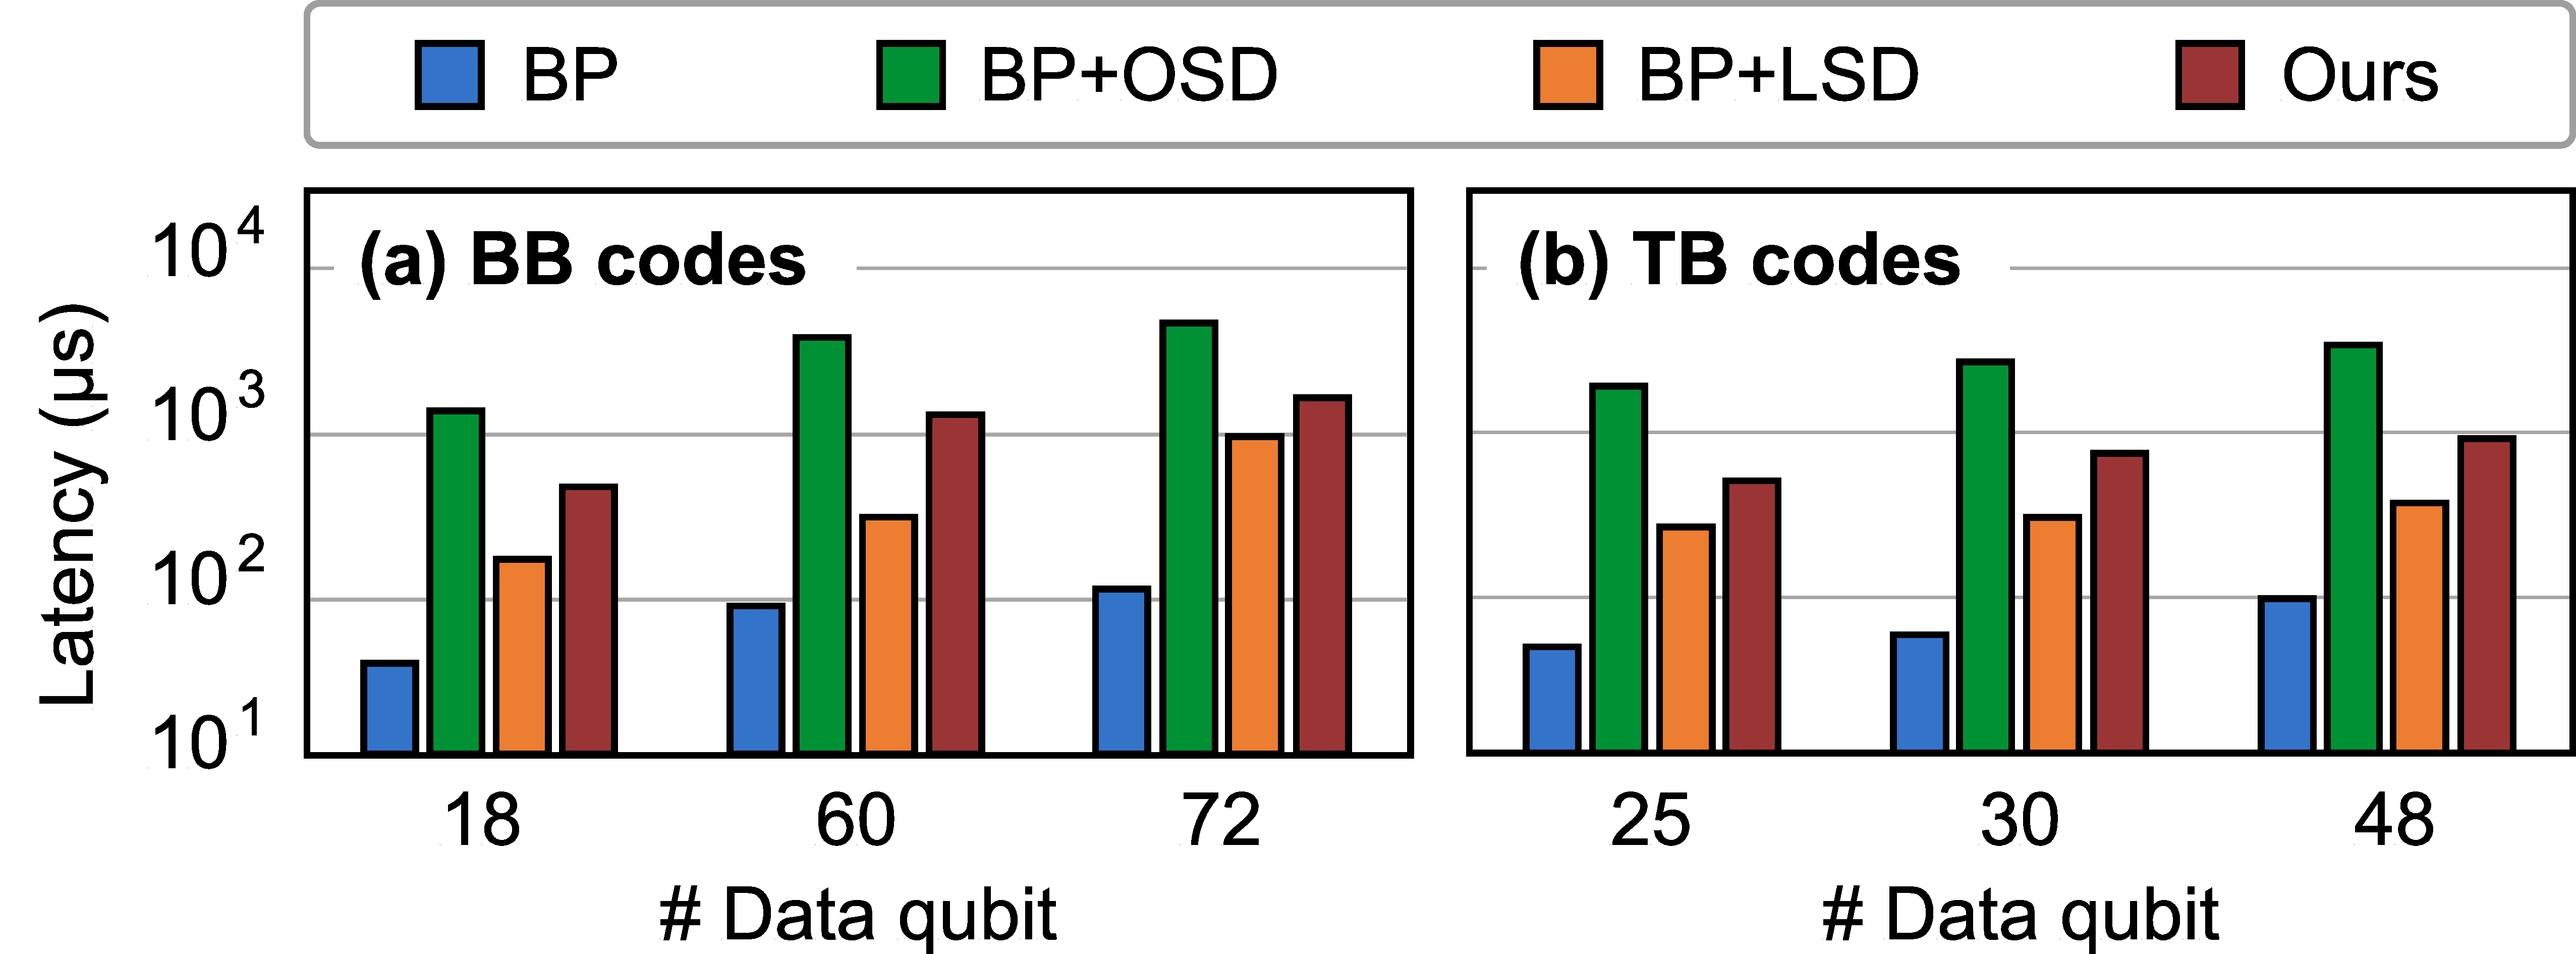
\includegraphics[width=1.0\columnwidth]{figures/Evaluation/latency.pdf}}
\vspace{-0.3cm}
\caption{Decoding latency of BP \cite{bp}, BP+OSD \cite{bposd}, BP+LSD \cite{bplsd}, and \papername on (a) BB codes and (b) TB codes, respectively.}
\vspace{-0.2cm}
\label{fig:latency}
\end{figure}

% \textbf{Logical error rate}.
As shown in \autoref{fig:LER_exp}, \papername reduces $1.55\sim 112\times$ logical error rate compared to prior decoders such as the state-of-the-art BP+OSD decoder. The maximum virtual bond of matrix product states in \papername is set to $\chi=16$. In particular, \papername achieves average $12.5\times$ logical error rate reduction on BB code [[18,4,4]], TB code [[30,6,4]], TB code [[48,4,8]]. Especially in TB code [[48,4,8]], the \papername has a logical error with $10^{-8}$ in physical error rate $10^{-3}$, which is $112\times$ lower than that of BP+OSD decoder.
% We also notice that the BP+LSD has achieved a similar logical error rate to that of BP+OSD, as claimed. The BP decoder has the highest logical error rate, as it often fails to converge due to degeneracy. 
Besides, we observe that the logical error rate curve of \papername has a larger slope than other decoders, which means \papername improved the error suppression capacity of qLDPC codes.

We compare \papername with recent qLDPC decoders, namely Vegapunk \cite{zhou2025vegapunk} and RelayBP \cite{relaybp}. Vegapunk achieves accuracy comparable to BP+OSD and BP+LSD, with higher performance on some codes, such as TB code [[30,6,4]], due to its decoupling strategy and greedy decoding. RelayBP, recently proposed by IBM, outperforms existing baselines through a relay ensembling technique that enhances BP’s robustness against trapping sets. In contrast, \papername delivers an average accuracy improvement of $1.97\times \sim 13.6\times$ over Vegapunk and $1.67\times \sim 10.5\times$ over RelayBP across various BB codes and TB codes. On BB code [[18,4,4]], \papername matches exact MLD almost perfectly, demonstrating its near-exact decoding. We do not extend this comparison to larger codes because the GPU memory required for exact MLD exceeds the capacity of our hardware. The remarkable decoding accuracy of \papername is due to its foundation in the principle of maximum likelihood decoding, which offers an accuracy advantage over other minimum weight decoders. Additionally, \papername utilizes the spin glass model to compress the search space of maximum likelihood decoders, thereby improving the success rate of identifying the most likely logical error.

% We also compare \papername with recent proposed qLDPC decoders, i.e., Vegapunk \cite{zhou2025vegapunk} and RelayBP \cite{relaybp}. We observe that Vegapunk achieves decoding accuracy comparable to BP+OSD and BP+LSD, with even higher accuracy on some codes, such as TB code [[30,6,4]]. The decoding performance of Vegapunk stems from its decoupling strategy and greedy decoding algorithm. Meanwhile, RelayBP, recently proposed by IBM, outperforms all existing baselines, primarily because its relay ensembling technique enhances the robustness of BP against trapping sets. Compared with Vegapunk and RelayBP, \papername delivers an average accuracy improvement of $1.97\times \sim 13.6\times$ and $1.67\times \sim 10.5\times$ across varying BB codes and TB codes. To further evaluate the accuracy of \papername, we compare \papername with exact MLD decoding on the BB code [[18,4,4]], as shown in \autoref{fig:LER_exp} (a). We find that the LER of \papername matches the exact MLD almost perfectly, demonstrating that \papername can realize near-exact qLDPC decoding. We do not extend this comparison to larger codes because the GPU memory required for exact MLD exceeds the capacity of our hardware.
% The remarkable decoding accuracy of \papername is due to its foundation in the principle of maximum likelihood decoding, which inherently offers an accuracy advantage over other minimum weight decoders. Additionally, \papername utilizes the spin glass model to compress the search space of maximum likelihood decoders, thereby improving the success rate of identifying the most likely logical error.





% \begin{figure}[t]
% \centerline{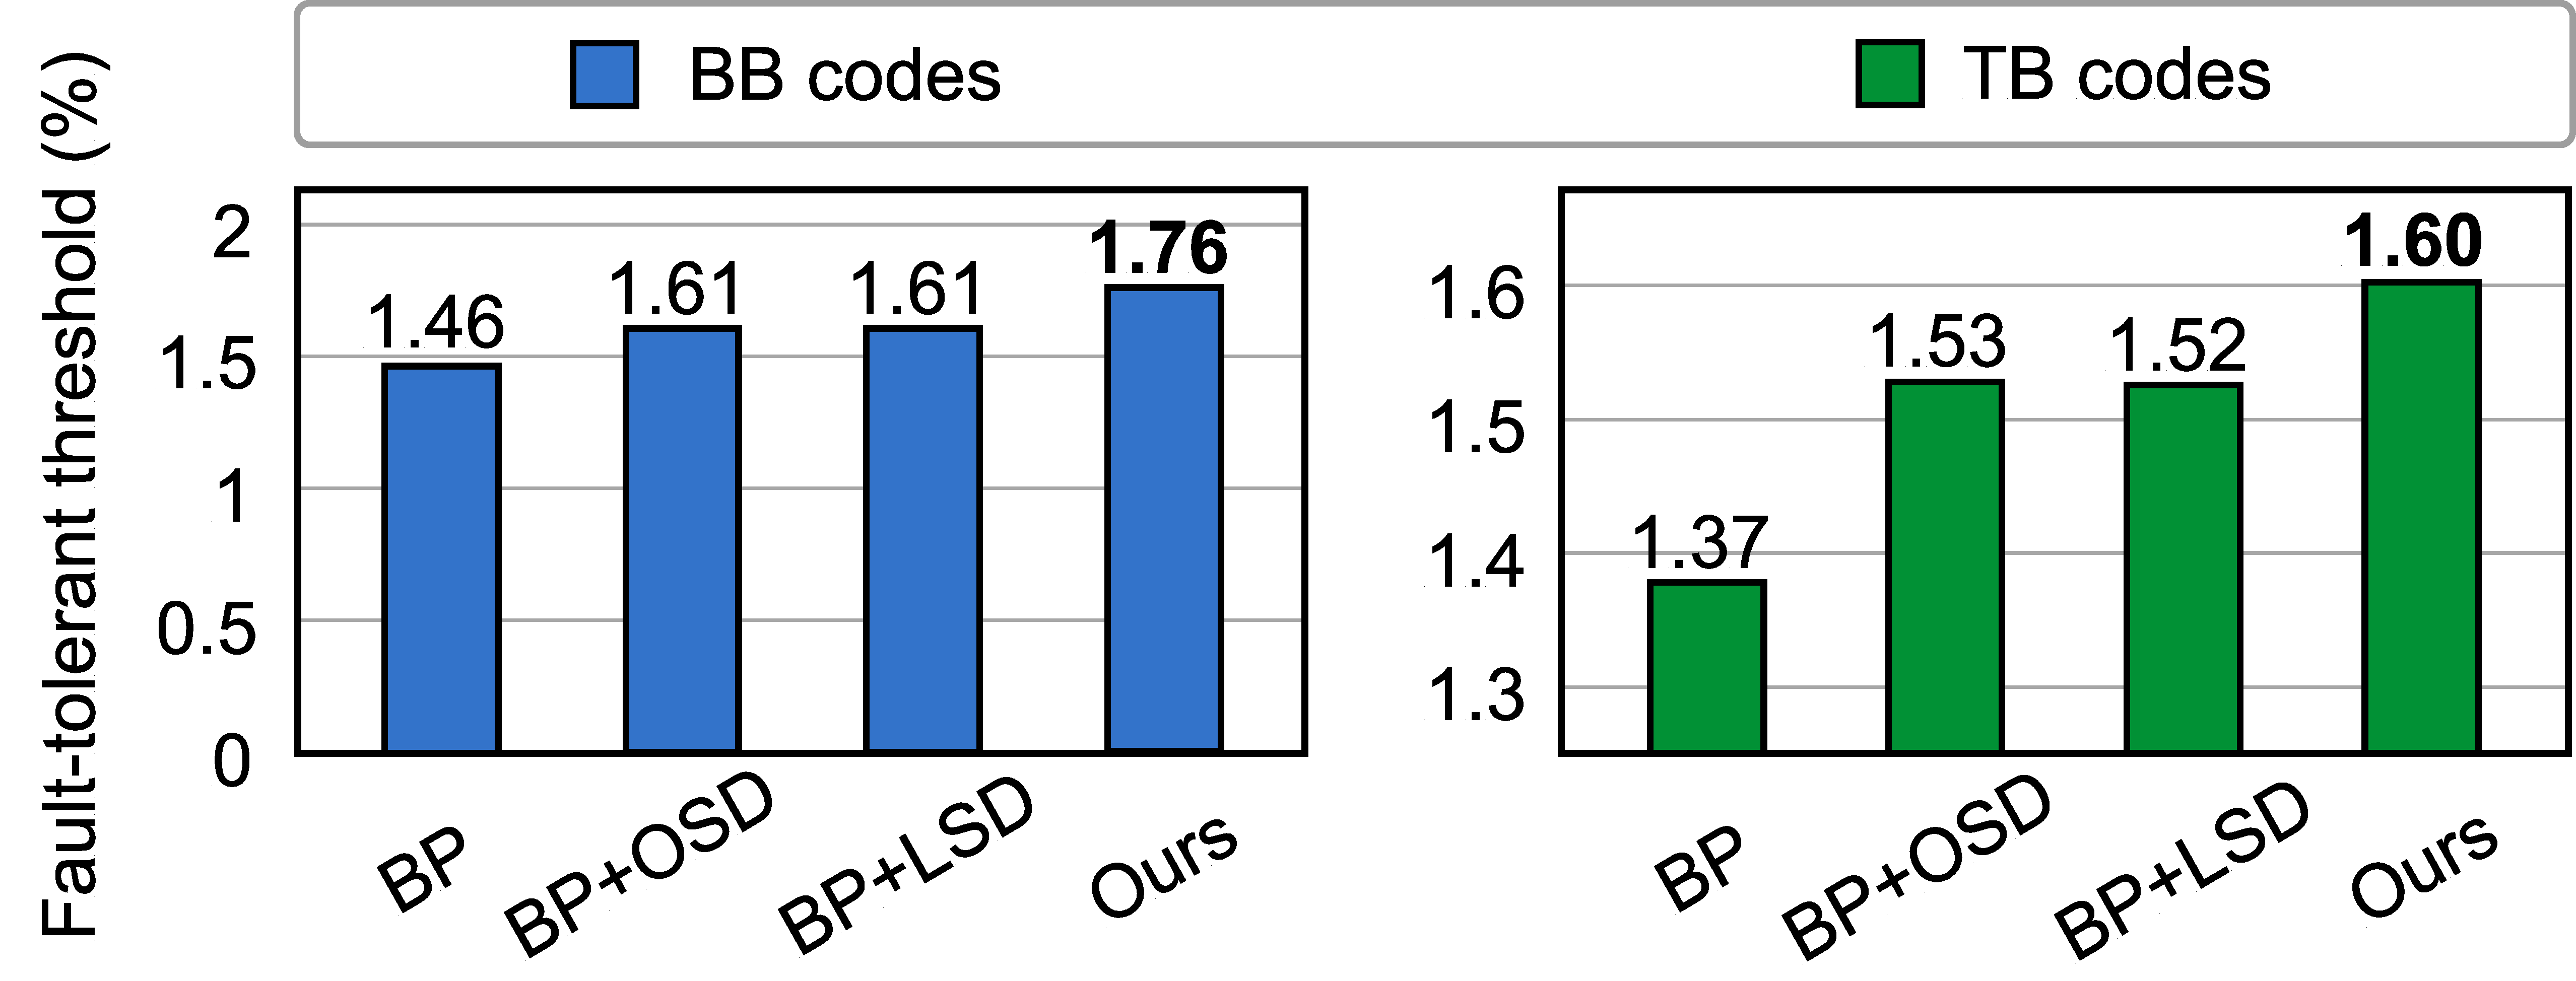
\includegraphics[width=1.0\columnwidth]{figures/Evaluation/fault_tolerant_threshold.pdf}}
% \vspace{-0.2cm}
% \caption{Fault-tolerant thresholds of BP \cite{bp}, BP+OSD \cite{bposd}, BP+LSD \cite{bplsd}, and \papername, respectively.}
% \vspace{-0.2cm}
% \label{fig:fault_tolerant_thresold}
% \end{figure}

% \textbf{Fault-tolerant threshold}.
% We calculate the fault-tolerant threshold of different decoders in different code types using the data in \autoref{fig:LER_exp}. The fault-tolerant thresholds are shown in \autoref{fig:fault_tolerant_thresold}. \papername outperforms other decoders in both BB codes and TB codes with thresholds of $1.76\%$ and $1.60\%$, respectively. The thresholds of BP+OSD and BP+LSD are similar and lower than \papername by $0.15\%$ and $0.08\%$ in BB codes and TB codes, respectively. BP has the lowest performance, which is lower than  \papername by $0.30\%$ and $0.23\%$. The high fault-tolerant threshold of \papername means that it has a higher fault-tolerance ability compared with other minimum weight decoders. \papername also improves the deployability of qLDPC codes on quantum hardware, since reducing the physical error rate in hardware takes much more effort than designing better codes. Notice that the higher fault-tolerant threshold does not imply higher logical error rates. Around the fault-tolerant threshold, the logical error rate of \papername is still lower than that of other decoders.



\subsection{Decoding Performance}

\textbf{Decoding latency}.
\autoref{fig:latency} plots the average decoding latency of different decoders. Latency of \papername ranges from $447\sim 1599 \mu s$, which is $3.37\times$ lower than the BP+OSD decoder on average. BP and BP+LSD have a lower latency than \papername since they leverage the message passing parallelism and localised statistics to accelerate decoding. Considering the excellent decoding accuracy of \papername, the longer latency than BP and BP+LSD is acceptable. Additionally, the latency growth of \papername over code size exhibits a linear trend, as \papername employs parallel marginal probability calculation to enhance parallelism in the decoding process. The complexity of \papername is linear with the number of logical qubits and syndrome qubits.

% Required packages:
% \usepackage{multirow}
% \usepackage{makecell}
% \usepackage{booktabs}

\begin{table}[t]
\centering
\renewcommand{\arraystretch}{1.25}
\caption{Tensor Compression of \papername.}
\label{tab:exp_tensor_compression}
\resizebox{\linewidth}{!}{
\begin{tabular}{c|l|lll|lll}
\toprule
\multirow{2}{*}{}& \makecell[l]{\textbf{Code}\\\textbf{type}}  &
\multicolumn{3}{c|}{\textbf{BB codes}} & \multicolumn{3}{c}{\textbf{TB codes}}  \\ \cline{2-8}
 & \makecell[l]{\textbf{Code}\\\textbf{size}} &
18 & 60 & 72 & 25 & 30 & 48 \\ \hline
% \midrule

% ================= COMPUTATION WORKLOAD ===================
\multirow{3}{*}{
\rotatebox{90}{%
    \parbox[c][.1cm][c]{2cm}{%
      \centering \textbf{FLOPS}%
    }%
  }%
}
 & \makecell[l]{{Exact}\\{MLD}}&
8.9K & 2.4G & 6.1T & $6.2$P & $10^3$P & $10^7$P \\ \cline{2-8}

 & \makecell[l]{Tensor\\MLD} &
640 & 5.6K & 49K & 320 & 2.0K & 131K \\ \cline{2-8}

 & \makecell[l]{Reduc-\\tion($\times$)} &
$14.2$ &
$10^{5}$ &
% $4.2\times10^{5}$ &

$10^{8}$ &
% $1.3\times10^{8}$ &

$10^{13}$ &
% $1.9\times10^{13}$ &
$10^{15}$ &
% $3.4\times10^{15}$ &
% $1.1\times10^{17}$
$10^{17}$
\\ \hline



% ================= NUMBER OF TENSORS ===================
\multirow{3}{*}{
\rotatebox{90}{%
\parbox[c][.1cm][c]{2cm}{%
      \centering \textbf{\#Tensor}%
    }%
    }
}
 & \makecell[l]{{Exact}\\{MLD}} &
40 & 128 & 156 & 52 & 63 & 102 \\ \cline{2-8}

 & \makecell[l]{Tensor\\MLD} &
11 & 34 & 42 & 14 & 15 & 26 \\  \cline{2-8}

 & \makecell[l]{Reduc-\\tion($\times$)} &
3.6& 3.8& 3.7&
3.7& 4.2& 3.9\\  \hline

% ================= MAX TENSOR SIZE ===================
\multirow{3}{*}{\rotatebox{90}{\makecell[c]{\textbf{Max tensor} \\\textbf{size}}}}
 & \makecell[l]{{Exact}\\{MLD}} &
4.0K & 0.1M & 0.5M & 8.1K & 0.2M & 1.0M \\ \cline{2-8}

 & \makecell[l]{Tensor\\MLD} &
512 & 512 & 512 & 512 & 512 & 512 \\ \cline{2-8}

 & \makecell[l]{Reduc-\\tion($\times$)} &
8& 256& 1024&
16& 512& 2048\\\hline
\multirow{4}{*}{
\rotatebox{90}{%
\parbox[c][.1cm][c]{2cm}{%
      \centering \textbf{Memory Footprint}%
    }%
    }
}
 & \makecell[l]{\textbf{Code}\\\textbf{size}} & 108      & 144      & 288      & 126      & 180      & 254      \\  \cline{2-8}

%  & \makecell[l]{\textbf{Code}\\\textbf{size}} &
% 18 & 60 & 72 & 25 & 30 & 48 \\ \hline

 & \makecell[l]{{Exact}\\{MLD}}  & 20KB    & 54KB    & 2.6MB  & 1.3MB  & 39MB & 3.9GB \\ \cline{2-8}
 & \makecell[l]{Tensor\\MLD}    & 1.1KB     & 1.4KB     & 2.8KB     & 4.0KB     & 6.0KB     & 8.7KB     \\ \cline{2-8}
 & \makecell[l]{Reduc-\\tion($\times$)}  & 18.2 & 36.7 & 914.5 & 333.3 & 6462 & 450176 \\
\bottomrule
\end{tabular}
}
\end{table}









% \begin{table*}[t]
% \centering
% \renewcommand{\arraystretch}{1.25}
% \caption{Tensor Compression of \papername.}
% \label{tab:exp_tensor_compression_transposed}

% % \resizebox{\textwidth}{!}{
% \begin{tabular}{
% l c
% |ccc
% |ccc
% |ccc
% }
% \toprule
% \textbf{Code type} &
% \makecell[c]{\textbf{Code}\\\textbf{size}} &
% \multicolumn{3}{c|}{\textbf{FLOPS}} &
% \multicolumn{3}{c|}{\textbf{\#Tensor}} &
% \multicolumn{3}{c}{\textbf{Max tensor size}} \\ \cline{3-11}
%  & & Exact & Tensor & Red. ($\times$) & Exact & Tensor & Red. ($\times$) & Exact & Tensor & Red. ($\times$) \\
% \midrule

% \multirow{3}{*}{BB codes}
%  & 18 &
% 8.9K & 640 & 14.2 &
% 40 & 11 & 3.6 &
% 4.0K & 512 & 8 \\ \cline{2-11}

%  & 60 &
% 2.4G & 5.6K & $10^{5}$ &
% 128 & 34 & 3.8 &
% 0.1M & 512 & 256 \\ \cline{2-11}

%  & 72 &
% 6.1T & 49K & $10^{8}$ &
% 156 & 42 & 3.7 &
% 0.5M & 512 & 1024 \\ 
% \midrule

% \multirow{3}{*}{TB codes}
%  & 25 &
% 6.2P & 320 & $10^{13}$ &
% 52 & 14 & 3.7 &
% 8.1K & 512 & 16 \\ \cline{2-11}

%  & 30 &
% $10^{3}$P & 2.0K & $10^{15}$ &
% 63 & 15 & 4.2 &
% 0.2M & 512 & 512 \\ \cline{2-11}

%  & 48 &
% $10^{7}$P & 131K & $10^{17}$ &
% 102 & 26 & 3.9 &
% 1.0M & 512 & 2048 \\

% \bottomrule
% \end{tabular}
% % }
% \end{table*}


\textbf{Tensor compression}. \autoref{tab:exp_tensor_compression} quantifies the complexity-accuracy tradeoff of \papername, highlighting the effectiveness of our tensor decomposition and compression. The results demonstrate a super-exponential reduction in computational workload (FLOPS) compared to Exact MLD. For instance, for the BB code [72,12,6]], \papername reduces the workload from 6.1 TFLOPS to just 49 KFLOPS. This advantage scales dramatically, achieving a $10^{17}\times$ reduction for the TB code [[48,4,8]].
In addition to computational gains, \papername significantly reduces memory requirements. The total number of tensors (\#Tensor) is consistently reduced by a factor of $3.6\times \sim 4.2\times$ across all codes. More critically, the Max Tensor Size, which represents the primary memory bottleneck, is shrunk from an exponentially growing value (e.g., 1.0M for the TB code [[48,4,8]]) to a small, constant 512. Considering this massive reduction in both computation and memory with little accuracy loss, \papername proves to be a highly efficient and scalable solution.





\subsection{Ablation Study}

In this section, we study the memory and computation cost of using different optimization techniques. We measure three different tensor network states, including the full tensor network without any
optimization, the matrix product state (MPS) with exact decomposition, and a 1D-chain matrix product state with offline contraction optimization. The metrics include storage memory for storing the tensor network, the Number of Floating Operations needed for tensor network contraction, and the Maximum Tensor Size when contracting the tensor network.

\textbf{Memory footprint.}
\autoref{fig:ablation_study}~(a)  shows the memory requirements for different tensor network states. After exact decomposition and offline contraction, 1D-chain MPS saves an average $9.1\times$ memory usage compared with the full tensor network, which consumes $5.2$KB memory on average. This trend is expected because the full tensor network, in its unoptimized form, represents a high-rank tensor whose memory consumption can be exponential in the worst case, whereas the 1D-chain MPS uses linear amounts of low-rank tensors.
We also find that only the MPS with exact decomposition has an average $39.1$KB memory usage, which is higher than the full tensor network. 
% This is because the exact decomposition decomposes the high-rank tensor with low-rank MPS, thereby increasing the number of tensors. Since the dimension $n$ of the original tensor equals the column sparsity of the check matrix, which is small in qLDPC codes, the reduction from $O(2^n)$ to $O(8n)$ is not remarkable.


\textbf{Number of floating operations.}
\autoref{fig:ablation_study}~(b) illustrates the number of floating operations required for tensor network contraction. The full tensor network demands $2.3\times10^{21}$  FLOPs, representing the highest computational burden. This contrasts sharply with MPS (with exact decomposition), which requires an average $8.0\times10^8$ FLOPs, and the 1D-chain matrix product state further reduces the computation cost to $3.1\times 10^4$ FLOPs, which is $7.3\times 10^{16}$ lower than the full tensor network. 
% The significantly higher FLOPs for the full tensor network stem from its inherently exponential worst-case computation complexity and the NP-hard problem of finding an optimal contraction path. 
The MPS offers theoretical polynomial-time complexity for contraction, drastically improving efficiency. The 1D-chain MPS with offline optimization further optimizes this for online decoding, explicitly leveraging a \textit{partial tracing strategy} with a polynomial complexity O($M\chi^2+\log K\cdot K^2\chi^4$), which is notably efficient compared to enumerating all logical spins. This can be observed from the reduction times compared with the full tensor network. The 1D-chain MPS achieves a $14.2\times$ reduction on the BB code [[18,4,4]] and a $1.3\times 10^8 \times$ reduction on the BB code [[2,12,6]], which depicts an exponential reduction trend.

\begin{figure}[t]
\centerline{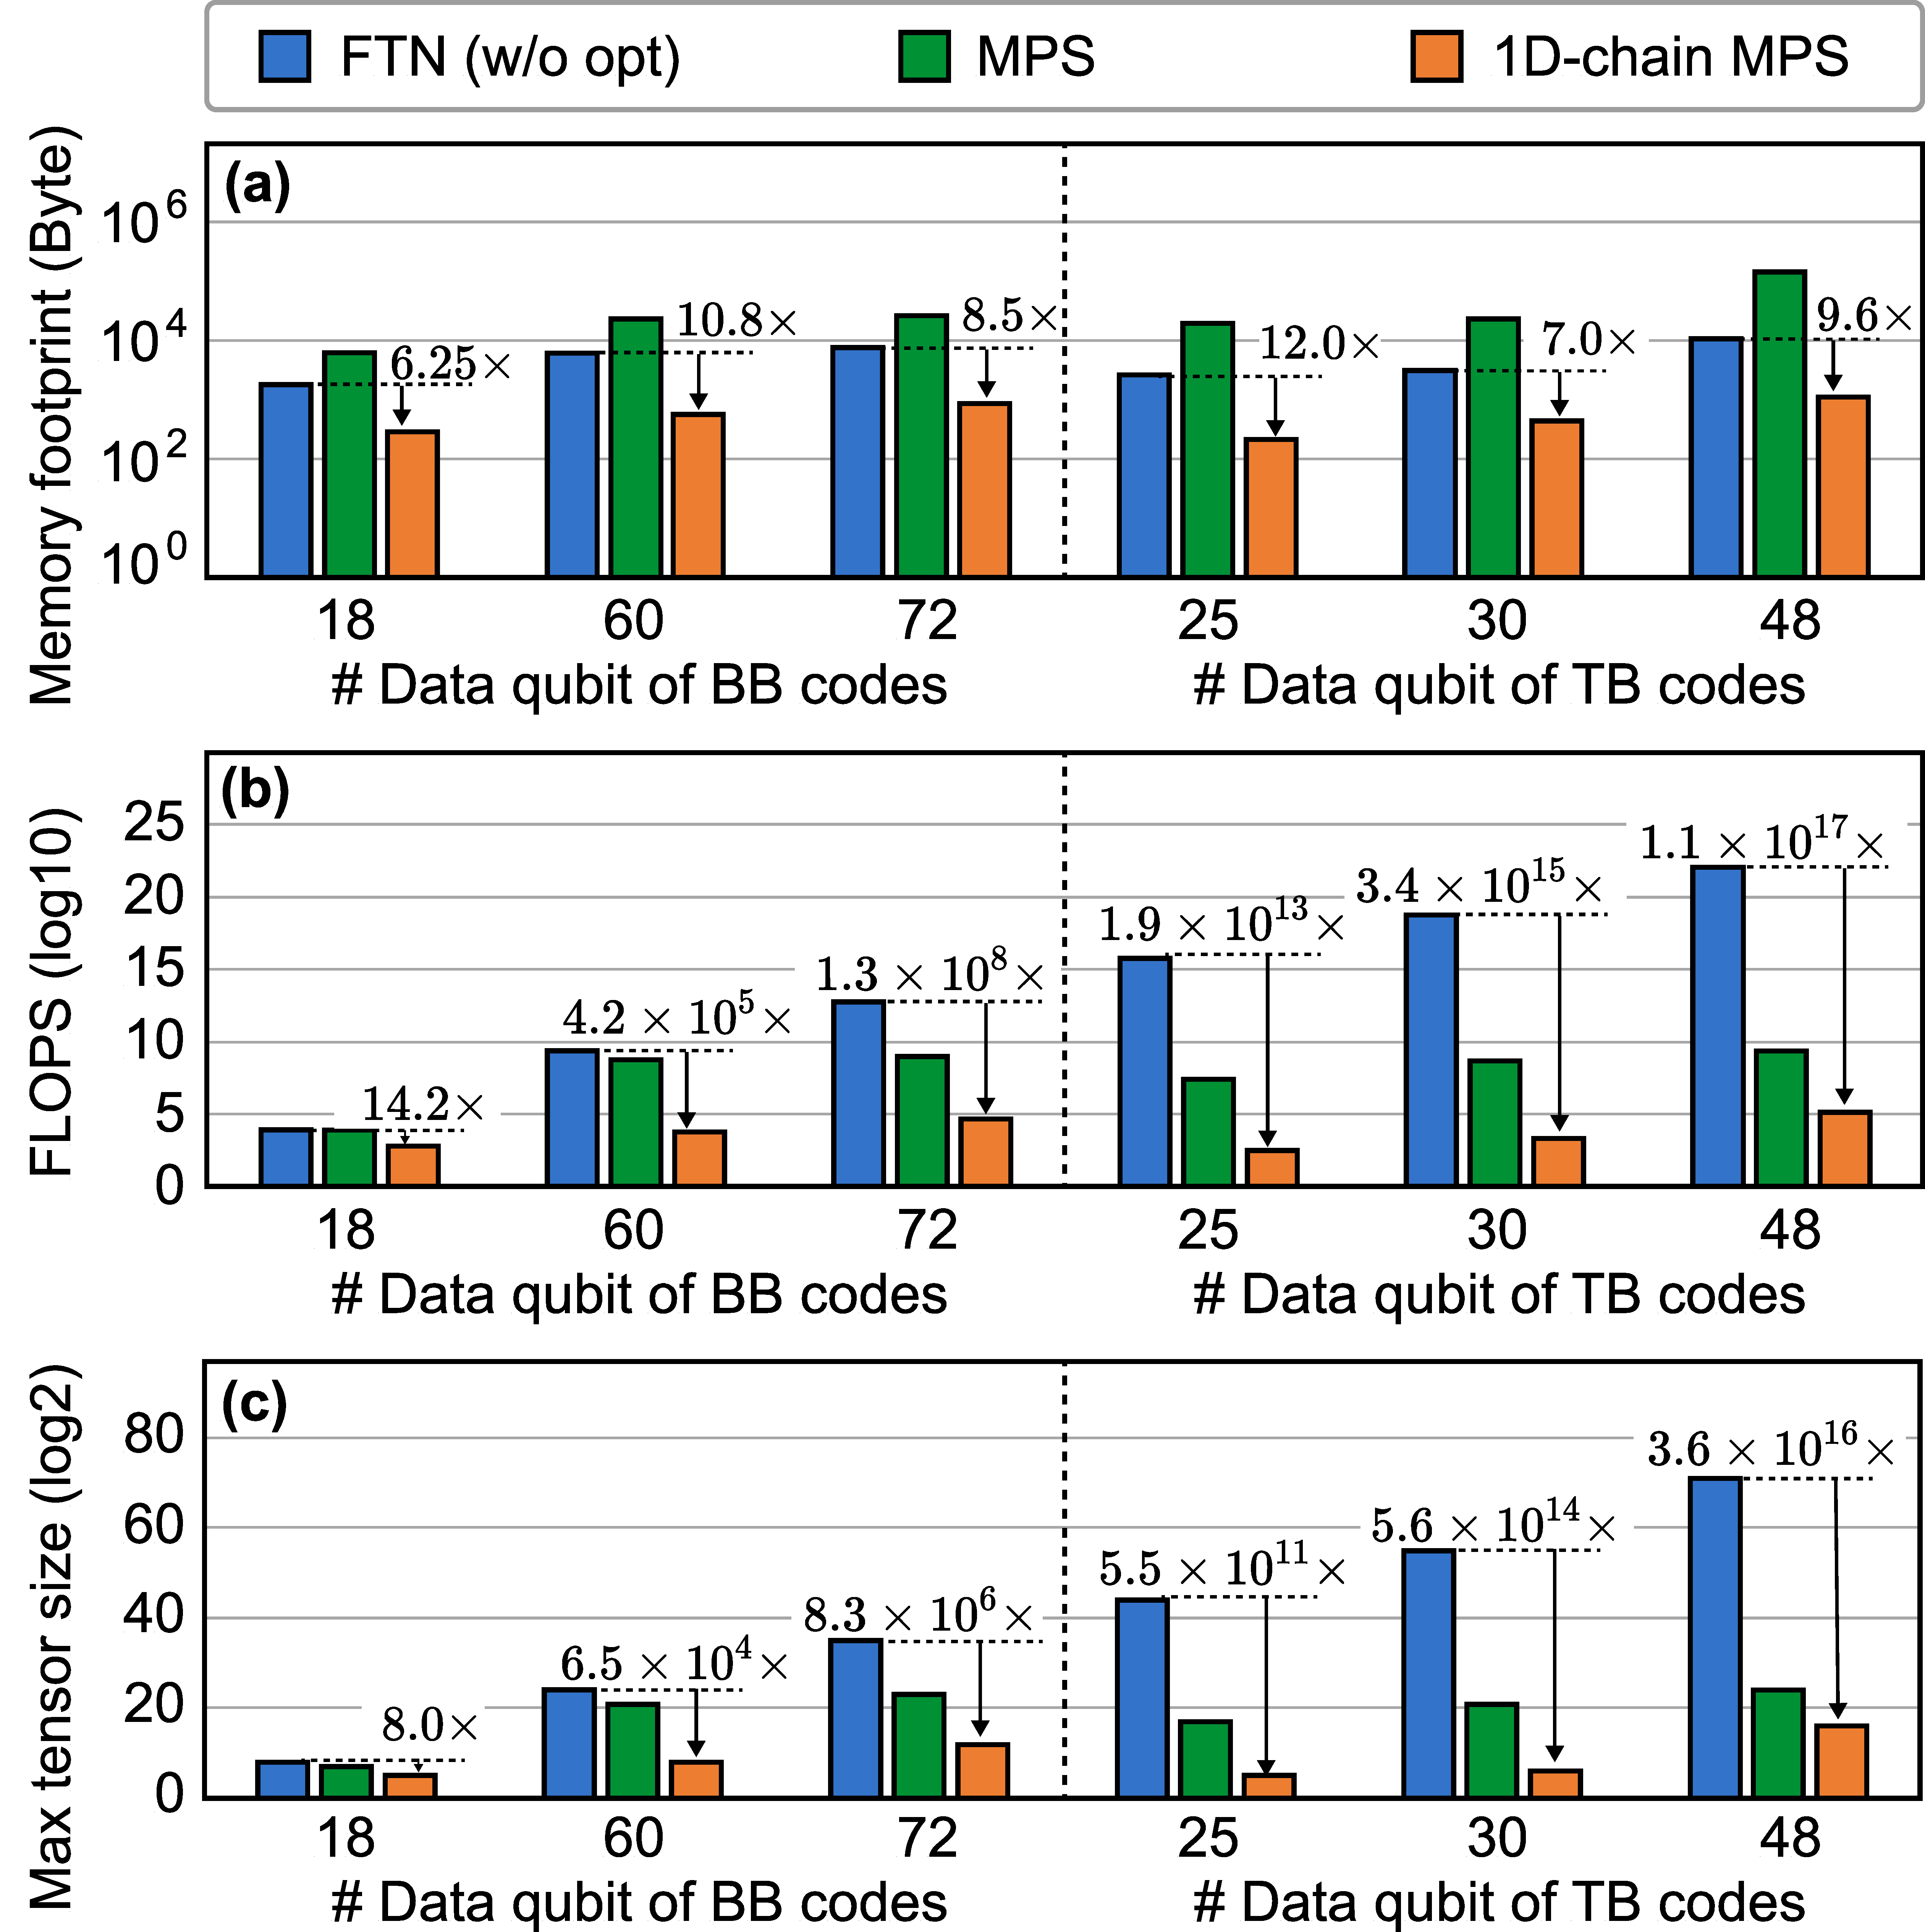
\includegraphics[width=1.0\columnwidth]{figures/Evaluation/ablation_study.pdf}}
\vspace{-0.3cm}
\caption{Ablation study of \papername.}
\vspace{-0.4cm}
\label{fig:ablation_study}
\end{figure}

\textbf{Maximum tensor size in computation.}
\autoref{fig:ablation_study}~(c) presents the maximum tensor size encountered during the contraction process. 1D-chain MPS achieves an $8\sim3.6\times 10^{16} \times$ reduction on maximum tensor size. The large maximum tensor size in the full tensor network is a direct consequence of the exponential growth of intermediate tensors during contraction. The peak tensor size, such as $2^{71}$ in TB code [[48,4,8]], often poses a memory bottleneck. The MPS fundamentally solves this by bounding intermediate tensor sizes, leading to a more manageable memory footprint in the contraction process. We can see that the maximum tensor size of a 1D-chain is always lower than $2^{20}$, which is a much lower memory than can be handled on classical devices.